\documentclass[11pt]{article}

\usepackage[a4paper, margin=2cm,headsep=6pt]{geometry}
\usepackage{lineno}
\usepackage[english]{babel}
\usepackage{graphicx}
\usepackage{float}
\newcommand{\soptitle}{Inferring ploidy number and testing for aneuploidy from next generation sequencing data}
\usepackage{fancyhdr}
\pagestyle{fancy}
\linespread{1.25}
\fancyhead[R]{CID 01383312}
\fancyhead[L]{Oliver Tarrant}
\usepackage{csquotes}
\usepackage[backend=bibtex,style=authoryear]{biblatex}
\bibliography{Project_ProposalBib.bib}
\begin{document}
\begin{titlepage}


\begin{center}
\hrule
\vspace{2pt}
\hrule
\vspace{2cm}
\LARGE {\bf \underline{Project Proposal}}\\
\vspace{2cm}
\huge{\bf \soptitle}\\
\vspace{4cm}
\LARGE {\bf Oliver Tarrant - CMEE MRes}\\
\vfill
\huge {\bf Supervisor - Dr. Matteo Fumagalli}\\
\LARGE {\bf Research Fellow, Department of Life Science}\\
\LARGE {\bf Imperial College London}\\
\large {\bf m.fumagalli@imperial.ac.uk}
\end{center}
\hrule
\vspace{2pt}
\hrule
\end{titlepage}
\linenumbers
{\bf Keywords: }\\ Next-generation sequencing, Genomics, Ploidy, bioinformatics,  Statistical genetics, Population Biology
\section{Introduction}
\paragraph{} Genomic sequencing has come a long way since the first sequenicing of a human genome was completed in 2001. Early Sanger sequencing techniques have now been replaced by modern high throughput sequencing technologies. These are all based on similar principles. Data is produced in the form of a collection of short reads of genetic information. Reads are then combined to build a genome by de novo, or if a reference genome already exists then they can be aligned to this \autocite{Jason2015}.
\paragraph{} With many financial and time pressures, researchers are usually restricted to sequencing at low depths. Problems then arise when trying to build a genome de novo. Particularly when trying to determine the ploidy of an organism. With only a low sequencing depth, it is likely that not all copies of a chromosome will be sequenced, especially when working with an organism with a high ploidy number \autocite{Nielsen2011}. When testing for aneuploidy (The presence of an abnormal number of chromosomes in a cell) or trying to infer ploidy number from low depth data these issues are amplified. It is likely many cases would get missed as either not all chromosomes would be read, or if there were less chromosomes present than expected then it may get interpretated as one of the chromosomes not being sequenced rather than it not existing.
\paragraph{} The current research for infering ploidy number from next generation sequencing data is based around tools which rely on use of hidden markov chain models (HMM) \autocite{Kai2007}. The model used has double emmision distributions where the use of the coverage and data observed for windows of loci on the genome are used to infer the unknown ploidy level. The relevent parameters and sequence of ploidy levels are then derived by using the expectation maximisation and viterbi algorithms respectively \autocite{Colella2007}. If two samples have different ploidy numbers then the probabilities used in the model to infer become unreliable and thus it is now needed to develop a test so that these aneuploidy cases are picked up. 
\paragraph{} I aim to apply the methods I develop to looking at the affect of ploidy on the virulence of the Bd (Batrachochytrium dendrobatidis) fungus. A recent increase in outbreaks of fungal diseases has caused havoc on many global species resulting in a strain on many vital food crops and putting many other species at risk of extinction. Bd fungus is a particularly important pathogen to study, infecting over 500 species of amphibians worldwide whilst having a mortality rate of almost 100\%. As a result half the worlds amphibian populations are now in decline with some areas of Central America already having lost 40\% of their amphibian species from the fungus \autocite{Fisher2012}.
\section{Proposed Methods}
\paragraph{} I will aim to address those problems mentioned above by building upon tools to infer ploidy and copy number variation and test for aneuploidy. Currently, tools such as QuantiSNP, use a HMM to test for aneuploidy but also involve a likelihood ratio test for testing if samples have the same ploidy level \autocite{Colella2007}. I will be looking for more computationally efficient ways of producing analytical approximations to such calculations. I will also work on techniques to improve our ability of infering ploidy states from low depth data. Development will use the general framework mentioned above in the form of the HMM. HMM's are widely used in research looking at copy number variation (CNV) and are the basis of tools such as CNAseg and PennCNV \autocite{Min2013, Kai2007}. I will aim to build upon these tools to improve the accuracy and flexibility, especially at low coverage. I may need to incorporate some methods from population genetics to deal with problems associated with cases with low sample numbers. I will test these models on simulated data before applying them to real data sets with the aim of determining the phenotypical affect of ploidy number in specific organisms. Specifically I will be using a gloablly representative sample set of 234 isolates of the Bd fungus \autocite{Ferrer2011} and try to associate ploidy changes with the virulence phenotype.
\section{Anticipated outcomes}
\paragraph{} This project will develop a test for aneuploidy for organisms given next generation sequenced data. It will also build on methods and develop further statistical tools allow us to more accurately infer the ploidy number of organisms that have been sequenced at low depths. These tools will allow me to produce beneficially results to look at whether or not the ploidy number has any affect in the phenotypical properties of specific organisms. 
\section{Feasibilty}
\paragraph{} The project will be split into three main sections: the development of a test for aneuploidy, improvements to methods to infer ploidy number from low depth data and applications of these tools to Bd fungus data. Below is a Gantt chart showing my proposed timeline and deadlines for my project.
\begin{figure}[H]
\begin{center}
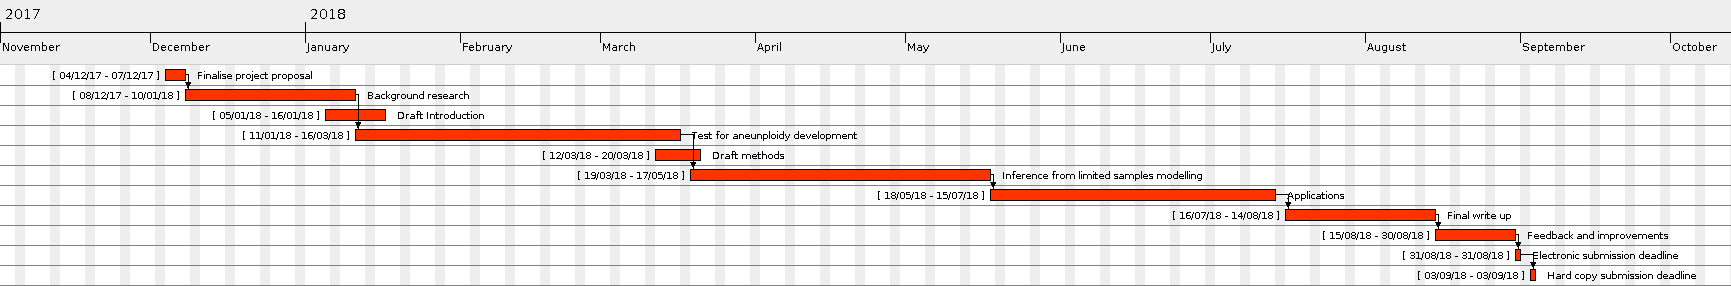
\includegraphics[scale=0.28]{GanttChart.png}
\end{center}
\end{figure}
\section{Budget}
\paragraph{} For this project I would like to request use of the \pounds 500 availible grant to cover the expenses of travel within my research. Whilst working with the Bd fungi  dataset I will be collaborating with associates based in St Mary's hospital in London. I have budgeted for approximately \pounds 150 at \pounds 15.20 per a return train ticket for this travel. I would also like to budget for a visit to our collaborators on the theory at the University of Copenhagen in Denmark. Flights and travel would come to approximately \pounds 150 and accomodation a further \pounds 200. I would like to commit any remaining budget to covering the costs of visiting conferences and seminars so that I can further my research and understanding in my area. This would allow me to make connections with research leaders and hopefully develop my project to a higher standard.
\pagebreak 
\printbibliography
\end{document}